
In this section two different solution approaches for mixed-integer non-linear programs (MINLP) will be presented.
The problem considered here in its most general form can be written as
\program{prog:stdMINLP}{
        & \minimize{x,y} & & C = f(x,y) \\
        & \st & & g_j(x,y) \leq 0, \; \; j \in \mathset{J} \\
        & & & x \in \mathset{X}, \; y \in \mathset{Y}
    }
where $\mathset{J}$ denotes the set of all constraints while $\mathset{X}$ and $\mathset{Y}$ denote the set 
of continuous and integer variables respectively. 
    
The main focus lies on discussing two alternative solution approaches to the aforementioned class of problems.
First the outer approximation algorithm, which is implemented in \gproms, is introduced.
Then then an alternative approach to solve this class of problems, based on a continuous reformulation of
the discrete decision variables, which has recently been proposed \cite{Kraemer.2010,Stein.2004} will also be
discussed. Both approaches will later be applied to the example process and compared in terms of optimality,
time consumption and robustness.

    \subsection{Outer approximaltion}
        The outer approximation (OA) algorithm relies on consecutively solving two sub-problems in order to
        converge to a solution. These problems are an NLP sub-problem, in which all integer values are fixed, 
        as well as a linearized version of the original MINLP \progref{prog:stdMINLP}. 
        
        First we consider the continuous sub-problem. Keeping all integer values constant
        results in the following NLP
        \program{prog:fixedyNLP}{
            & \minimize{x} & & C_{LB}^k = f(x,y^k) \\
            & \st & & g_j(x,y^k) \leq 0, \; \; j \in \mathset{J} \\
            & & & x \in \mathset{X}.
        }
        where the index $k$ denotes the values for the $k^{th}$ iteration. 
        If \progref{prog:fixedyNLP} is infeasible the NLP feasibility subproblem for fixed $y^k$ can be solved.
        \program{prog:feasibleNLP}{
            & \minimize{x} & & u \\
            & \st & & g_j(x,y^k) \leq u, \; \; j \in \mathset{J} \\
            & & & x \in \mathset{X}, \; \; u \in \mathbb{R}
        }
        This NLP returns a strictly positive value for $u$.

        Aside from the presented NLP's a linearized version of \progref{prog:stdMINLP} is regularly solved
        \program{prog:MILP}{
            & \minimize{x, y} & & C_L^k = \alpha \\
            & \st & & f(x^k,y^k) + \nabla f(x^k,y^k)^T \begin{bmatrix} x - x^k \\ y - y^k \end{bmatrix} \leq \alpha \\
            & & & g_j(x^k,y^k) + \nabla g_j(x^k,y^k)^T \begin{bmatrix} x - x^k \\ y - y^k \end{bmatrix} \leq 0, \; \; j \in \mathset{J} \\
            & & & x \in \mathset{X}, \; \; y \in \mathset{Y}, \; \; k = {1 \dots K}
        }
        The linearized problem can be constructed in several ways from the set of points $K$ attained in previous iterations.
        Sometimes only violated or active constraints are linearized. When objective function and constraints are convex, the
        objective function is underestimated, while the constraints are overestimated. From the overestimated constraints stems
        the name outer approximation.

        \begin{figure}
            \center
            \begin{tikzpicture}[scale=0.7]
    \pgfmathsetmacro{\blockh}{1.5cm}
    \pgfmathsetmacro{\blockw}{2.2cm}
    \tikzset{box/.style={draw, rectangle, minimum height=\blockh, minimum width=\blockw, align=center}}
	\node (A) [box] at (0,0) {NLP \\ \progref{prog:fixedyNLP}} ;
    \node (B) [box] at (6,0) {MILP \\ \progref{prog:MILP}} ; 
    \draw [arrow] (A.east) -- (B.west) ;
    \draw [arrow] ($(A.west) - (2,0)$) -- (A.west) ; 
    \draw [arrow] (B.east) -- ($(B.east) + (2,0)$) ;
    \draw [arrow] (B.south) -- ++(0,-1) -- ++($(A.south) - (B.south)$) -- (A.south) ; 
\end{tikzpicture}

            \caption{Outer approximation algorithm.}
            \label{fig:OA_algorithm}
        \end{figure}

        Each solution of the NLP with fixed $y^k$ yields a new point $(x^k,y^k)$ which is used to
        construct an updated version of the MILP. The MILP generally includes linearized versions of all constraints and
        the objective function. As more and more points become available during the iterative process, new constraints
        are constructed for each available point.

        The main theorem for the derivation of the OA algorithm states, that the optimal solution of the problem
        \progref{prog:MILP} constructed from all points $(x^k,y^k), k \in K^{\ast}$. Where $K^{\ast}$ is made up of
        all optimal solutions of \progref{prog:fixedyNLP} where the current $y^k$ yields a feasible solution, and
        \progref{prog:feasibleNLP} where infeasible solutions of the NLP with fixed $y^k$ are encountered. It should
        again be emphasized, that this theorem holds only for convex a objective function and constraints.

        As the points necessary to construct the aforementioned system are not available when the solution process
        commences, a smaller systems is constructed and extended as more points become available. Initially again
        the fully relaxed problem is solved. This again yields an absolute lower bound for the original problem. The solution of each consecutive
        MILP gives a new lower bound which will always be greater than the bounds from previous iterations. Without any
        prove this argument is supported by the fact that adding new linear constraints will limit the feasible region of
        the problem and hence further restrict the possible solutions for the continuous variables.

        The optimal points attained from the NLP subproblems with fixed discrete values form upper bounds on the optimal
        solution. Here no statement can be made about the quality of the bound in each step, but rather is the current
        upper bound updated, once a lower value is encountered.

        The iterative process terminates, once the current upper and lower bound are within a given tolerance. It can be
        pointed out, that the outer approximation algorithm converges to the optimal solution in a single iteration if
        objective function and constraints in the original problem are linear, since in that case problems
        \progref{prog:stdMINLP} and \progref{prog:MILP} are equivalent.



    \subsection{Continuous reformulation}
    \label{sec:opt:theory:continuous}
    An alternative approach to solving discrete-continuous problems is to reformulate them as NLP
    and introduce further constraints which ensure that the discrete decision variables will assume integer values.
    Several different authors have proposed ways of reformulating integer decisions. One common way is to introduce
    the so called complementary or equilibrium constraints which lead to problems that must be dealt with designated
    (NLP) solvers. Despite the fact that they posses poor theoretical features they have successfully been applied
    to problems of different scales. Lately however, alternative approaches have been suggested, which can be implemented
    in \gproms with relative ease and then solved with the NLP solvers included in the modeling environment.
    The first approach presented formulates a so called non-linear complementary problem (NCP) by introducing
    further constraints. Secondly within the distributed stream method, differentiable distribution functions (DDF)
    are formulated to model the associated integer decisions. In the following both approaches will be summarized briefly.
    A more detailed discussion of continuous reformulation techniques can be found in \cite{Stein.2004}.
    \begin{figure}
        \scriptsize
        \center
        \begin{subfigure}{0.48\textwidth}
            % GNUPLOT: LaTeX picture with Postscript
\begingroup
  \makeatletter
  \providecommand\color[2][]{%
    \GenericError{(gnuplot) \space\space\space\@spaces}{%
      Package color not loaded in conjunction with
      terminal option `colourtext'%
    }{See the gnuplot documentation for explanation.%
    }{Either use 'blacktext' in gnuplot or load the package
      color.sty in LaTeX.}%
    \renewcommand\color[2][]{}%
  }%
  \providecommand\includegraphics[2][]{%
    \GenericError{(gnuplot) \space\space\space\@spaces}{%
      Package graphicx or graphics not loaded%
    }{See the gnuplot documentation for explanation.%
    }{The gnuplot epslatex terminal needs graphicx.sty or graphics.sty.}%
    \renewcommand\includegraphics[2][]{}%
  }%
  \providecommand\rotatebox[2]{#2}%
  \@ifundefined{ifGPcolor}{%
    \newif\ifGPcolor
    \GPcolortrue
  }{}%
  \@ifundefined{ifGPblacktext}{%
    \newif\ifGPblacktext
    \GPblacktexttrue
  }{}%
  % define a \g@addto@macro without @ in the name:
  \let\gplgaddtomacro\g@addto@macro
  % define empty templates for all commands taking text:
  \gdef\gplbacktext{}%
  \gdef\gplfronttext{}%
  \makeatother
  \ifGPblacktext
    % no textcolor at all
    \def\colorrgb#1{}%
    \def\colorgray#1{}%
  \else
    % gray or color?
    \ifGPcolor
      \def\colorrgb#1{\color[rgb]{#1}}%
      \def\colorgray#1{\color[gray]{#1}}%
      \expandafter\def\csname LTw\endcsname{\color{white}}%
      \expandafter\def\csname LTb\endcsname{\color{black}}%
      \expandafter\def\csname LTa\endcsname{\color{black}}%
      \expandafter\def\csname LT0\endcsname{\color[rgb]{1,0,0}}%
      \expandafter\def\csname LT1\endcsname{\color[rgb]{0,1,0}}%
      \expandafter\def\csname LT2\endcsname{\color[rgb]{0,0,1}}%
      \expandafter\def\csname LT3\endcsname{\color[rgb]{1,0,1}}%
      \expandafter\def\csname LT4\endcsname{\color[rgb]{0,1,1}}%
      \expandafter\def\csname LT5\endcsname{\color[rgb]{1,1,0}}%
      \expandafter\def\csname LT6\endcsname{\color[rgb]{0,0,0}}%
      \expandafter\def\csname LT7\endcsname{\color[rgb]{1,0.3,0}}%
      \expandafter\def\csname LT8\endcsname{\color[rgb]{0.5,0.5,0.5}}%
    \else
      % gray
      \def\colorrgb#1{\color{black}}%
      \def\colorgray#1{\color[gray]{#1}}%
      \expandafter\def\csname LTw\endcsname{\color{white}}%
      \expandafter\def\csname LTb\endcsname{\color{black}}%
      \expandafter\def\csname LTa\endcsname{\color{black}}%
      \expandafter\def\csname LT0\endcsname{\color{black}}%
      \expandafter\def\csname LT1\endcsname{\color{black}}%
      \expandafter\def\csname LT2\endcsname{\color{black}}%
      \expandafter\def\csname LT3\endcsname{\color{black}}%
      \expandafter\def\csname LT4\endcsname{\color{black}}%
      \expandafter\def\csname LT5\endcsname{\color{black}}%
      \expandafter\def\csname LT6\endcsname{\color{black}}%
      \expandafter\def\csname LT7\endcsname{\color{black}}%
      \expandafter\def\csname LT8\endcsname{\color{black}}%
    \fi
  \fi
  \setlength{\unitlength}{0.0500bp}%
  \begin{picture}(4762.00,1926.00)%
    \gplgaddtomacro\gplbacktext{%
      \csname LTb\endcsname%
      \put(686,320){\makebox(0,0)[r]{\strut{} 0.0}}%
      \put(686,1027){\makebox(0,0)[r]{\strut{} 0.2}}%
      \put(686,1200){\makebox(0,0)[r]{\strut{} $\mu$}}%
      \put(686,1733){\makebox(0,0)[r]{\strut{} 0.4}}%
      \put(782,160){\makebox(0,0){\strut{} 0.0}}%
      \put(1489,160){\makebox(0,0){\strut{} 0.2}}%
      \put(2195,160){\makebox(0,0){\strut{} 0.4}}%
      \put(2902,160){\makebox(0,0){\strut{} 0.6}}%
      \put(3608,160){\makebox(0,0){\strut{} 0.8}}%
      \put(4315,160){\makebox(0,0){\strut{} 1.0}}%
    }%
    \gplgaddtomacro\gplfronttext{%
    }%
    \gplbacktext
    \put(0,0){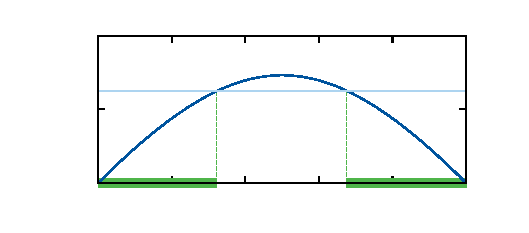
\includegraphics{GNUPlot/FB_Plot}}%
    \gplfronttext
  \end{picture}%
\endgroup

            \caption{plot of Fischer-Burmeister function.}
            \label{fig:FB_plot}
        \end{subfigure}
            \begin{subfigure}{0.48\textwidth}
            % GNUPLOT: LaTeX picture with Postscript
\begingroup
  \makeatletter
  \providecommand\color[2][]{%
    \GenericError{(gnuplot) \space\space\space\@spaces}{%
      Package color not loaded in conjunction with
      terminal option `colourtext'%
    }{See the gnuplot documentation for explanation.%
    }{Either use 'blacktext' in gnuplot or load the package
      color.sty in LaTeX.}%
    \renewcommand\color[2][]{}%
  }%
  \providecommand\includegraphics[2][]{%
    \GenericError{(gnuplot) \space\space\space\@spaces}{%
      Package graphicx or graphics not loaded%
    }{See the gnuplot documentation for explanation.%
    }{The gnuplot epslatex terminal needs graphicx.sty or graphics.sty.}%
    \renewcommand\includegraphics[2][]{}%
  }%
  \providecommand\rotatebox[2]{#2}%
  \@ifundefined{ifGPcolor}{%
    \newif\ifGPcolor
    \GPcolortrue
  }{}%
  \@ifundefined{ifGPblacktext}{%
    \newif\ifGPblacktext
    \GPblacktexttrue
  }{}%
  % define a \g@addto@macro without @ in the name:
  \let\gplgaddtomacro\g@addto@macro
  % define empty templates for all commands taking text:
  \gdef\gplbacktext{}%
  \gdef\gplfronttext{}%
  \makeatother
  \ifGPblacktext
    % no textcolor at all
    \def\colorrgb#1{}%
    \def\colorgray#1{}%
  \else
    % gray or color?
    \ifGPcolor
      \def\colorrgb#1{\color[rgb]{#1}}%
      \def\colorgray#1{\color[gray]{#1}}%
      \expandafter\def\csname LTw\endcsname{\color{white}}%
      \expandafter\def\csname LTb\endcsname{\color{black}}%
      \expandafter\def\csname LTa\endcsname{\color{black}}%
      \expandafter\def\csname LT0\endcsname{\color[rgb]{1,0,0}}%
      \expandafter\def\csname LT1\endcsname{\color[rgb]{0,1,0}}%
      \expandafter\def\csname LT2\endcsname{\color[rgb]{0,0,1}}%
      \expandafter\def\csname LT3\endcsname{\color[rgb]{1,0,1}}%
      \expandafter\def\csname LT4\endcsname{\color[rgb]{0,1,1}}%
      \expandafter\def\csname LT5\endcsname{\color[rgb]{1,1,0}}%
      \expandafter\def\csname LT6\endcsname{\color[rgb]{0,0,0}}%
      \expandafter\def\csname LT7\endcsname{\color[rgb]{1,0.3,0}}%
      \expandafter\def\csname LT8\endcsname{\color[rgb]{0.5,0.5,0.5}}%
    \else
      % gray
      \def\colorrgb#1{\color{black}}%
      \def\colorgray#1{\color[gray]{#1}}%
      \expandafter\def\csname LTw\endcsname{\color{white}}%
      \expandafter\def\csname LTb\endcsname{\color{black}}%
      \expandafter\def\csname LTa\endcsname{\color{black}}%
      \expandafter\def\csname LT0\endcsname{\color{black}}%
      \expandafter\def\csname LT1\endcsname{\color{black}}%
      \expandafter\def\csname LT2\endcsname{\color{black}}%
      \expandafter\def\csname LT3\endcsname{\color{black}}%
      \expandafter\def\csname LT4\endcsname{\color{black}}%
      \expandafter\def\csname LT5\endcsname{\color{black}}%
      \expandafter\def\csname LT6\endcsname{\color{black}}%
      \expandafter\def\csname LT7\endcsname{\color{black}}%
      \expandafter\def\csname LT8\endcsname{\color{black}}%
    \fi
  \fi
  \setlength{\unitlength}{0.0500bp}%
  \begin{picture}(4762.00,1926.00)%
    \gplgaddtomacro\gplbacktext{%
      \csname LTb\endcsname%
      \put(686,320){\makebox(0,0)[r]{\strut{} 0.0}}%
      \put(686,673){\makebox(0,0)[r]{\strut{} 0.4}}%
      \put(686,1027){\makebox(0,0)[r]{\strut{} 0.8}}%
      \put(686,1380){\makebox(0,0)[r]{\strut{} 1.2}}%
      \put(686,1733){\makebox(0,0)[r]{\strut{} 1.6}}%
      \put(782,160){\makebox(0,0){\strut{} 1}}%
      \put(1103,160){\makebox(0,0){\strut{} 2}}%
      \put(1424,160){\makebox(0,0){\strut{} 3}}%
      \put(1746,160){\makebox(0,0){\strut{} 4}}%
      \put(2067,160){\makebox(0,0){\strut{} 5}}%
      \put(2388,160){\makebox(0,0){\strut{} 6}}%
      \put(2709,160){\makebox(0,0){\strut{} 7}}%
      \put(3030,160){\makebox(0,0){\strut{} 8}}%
      \put(3351,160){\makebox(0,0){\strut{} 9}}%
      \put(3673,160){\makebox(0,0){\strut{} 10}}%
      \put(3994,160){\makebox(0,0){\strut{} 11}}%
      \put(4315,160){\makebox(0,0){\strut{} 12}}%
    }%
    \gplgaddtomacro\gplfronttext{%
    }%
    \gplbacktext
    \put(0,0){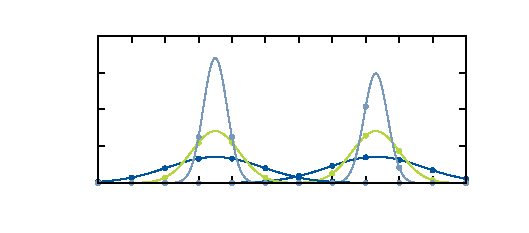
\includegraphics{GNUPlot/DDF_Plot}}%
    \gplfronttext
  \end{picture}%
\endgroup

            \caption{plot of DDF function.}
            \label{fig:DDF_plot}
        \end{subfigure}
    \end{figure}
    \todo{axis label for ddf and fb plot}

        \subsubsection{Non-linear complementary problem (NCP)}
        To arrive at a formulation with favourable theoretical properties Kraemer et al. \cite{Kraemer.2009} proposed
        a continuous reformulation based on the Fischer-Burmeister function
        \Eq{eq:opt:FB}{
            1 - \sqrt{y_i^2 + (1 - y_i)^2} = 0.
        }
        The zero set of this function contains exactly the values zero and and hence forces a continuous variable to
        take either integer value. However it is still very hard to solve complex, large-scale problems by simply
        enforcing this constraint. In order to facilitate convergence, the FB-function can be relaxed to a fully
        continuous problem
        \Eq{eq:opt:FB}{
            1 - \sqrt{y_i^2 + (1 - y_i)^2} \leq \mu.
        }
        The relaxation factor $\mu$ is then gradually reduced to zero in a sequence of NLP problems. \Figref{fig:FB_plot}
        shows a plot of the FB-function over the domain zero to one. The green lines on the x-axis denote the feasible domain
        for a given value of $\mu$. As one can see, if the relaxation factor is chosen large enough the entire span
        between zero and one is feasible, while for decreasing values the feasible set becomes disjunct and continuous
        variables are forced to either side to take on integer values.

        \subsubsection{Differentiable distribution function (DDF)}
        An alternative way of reaching a continuous formulation was brought fourth by Lang and Biegler \cite{Lang.2002}
        who within their distributed stream method propose the introduction of a differentiable distribution function (DDF)
        \Eq{}{
            \Psi_j = \frac{ \exp\left[ - \left( \frac{j - \sum_i \zeta_i i}{\sigma} \right)^2 \right] }{
                \sum_k \exp\left[ - \left( \frac{k - \sum_i \zeta_i i}{\sigma} \right)^2 \right]}.
        }
        This function models a normal distribution around a central tray. As the standard deviation ($\sigma$) is reduced,
        the spike at a given tray becomes more significant. Again in a series of NLP's $\sigma$ is driven to small value.
        At $\sigma = 0.25$ one can numerically consider the solution as integer. \Figref{fig:DDF_plot} shows a plot
        of the DDF function for a continuous stage value of 4.5 and 9.3 at $\sigma = 2, 1, 0.5$. Please note, that the
        values for each stage, denoted by dots, must add up to one. Depending on the distribution, a continuous plot can take
        on values larger than one.
